\chapter{Predicting conversions in display advertising based on URL embeddings}
Reference~\url{http://papers.adkdd.org/2020/papers/adkdd20-qiu-predicting.pdf}

\section{Какую задачу решают авторы?}

Авторы решают задачу предсказания вероятности конверсии пользователя для \textbf{конкретного} рекламодателя. \\

Интересной особенностью данной работы является то, что в качестве данных пользователя используется только история его активности в интернете --- последовательность URL'ов, которые посетил пользователь. \\

Решение можно разбить на две части:
\begin{itemize}
    \item Обучение векторных представлений для URL'ов
    \item Обучение модели, которая используя представления для URL'ов, предсказывает вероятность конверсии
\end{itemize}

Так как две части по сути независимы друг от друга, то в работе рассматриваются разные варианты для решения каждой из подзадач, и то какие из комбинаций решений являются наиболее хорошими.

\section{Как решают?}

Рассмотрим сначала решение каждой из подзадач по отдельности, и начнем с того как авторы предлагают получать векторные представления для URL'ов.

\subsection{URL Representation Schemes}

По аналогии с задачами NLP, авторы предлагают рассматривать последовательность URL'ов как документ, предложениями в котором являются последовательности токенов из URL'ов.

Причем каждый URL состоит максимум из трех токенов, например, \url{https://en.wikipedia.org/wiki/Main_Page/Some\_Subpage} разбивается на следующие токены
  [en.wikipedia.org, wiki, Main\_Page]. \\

Все способы, которые рассматриваются в работе можно поделить на две группы i) one-hot encoding ii) обучение эмбеддинов

\paragraph{One-hot encoding} Вектор для URL'a получается усреднением one-hot векторов токенов, на которые разбит URL.

Так как данный способ не позволяет учитывать семантическую похожесть между URL'ами и размер представления линейно зависит от числа токенов, то авторы рассматривают данный способ в качестве baseline решения.

\paragraph{Embedding learning} В рамках данного способа авторы предлагают использовать подход похожий на \texttt{Word2Vec (Skip-Gram with Negative Sampling)} с той лишь разницей, что обучаются эмбеддинги не для URL'ов целиком, но для токенов. \\

В качестве данных для обучения используют истории пользовательской активности. В результате, URL'ы, которые часто оказываются рядом в сессиях находятся близко друг к другу в векторном пространстве. \\

Для того чтобы из токенов получить векторное представление URL'a, в работе рассматривают следующие варианты
\begin{itemize}
    \item \texttt{Token\_concat} --- конкатенация векторов токенов
    \item \texttt{Token\_avg} --- усреднение векторов токенов
    \item \texttt{Domain\_only} --- используется только вектор домена (первый токен)
\end{itemize}

\subsection{Conversion Prediction}

Для того чтобы обучить, например, логистическую регрессию для предсказания вероятности конверсии, нужно истории пользователей превратить в фичи (вектор фиксированной длины). \\

Авторы статьи предлагают несколько вариантов того как это можно сделать
\begin{itemize}
    \item Усреднение векторов эмбеддингов из истории пользователя
    \item Однослойная нейросеть поверх усреднения векторов
    \item Так как предыдущие варианты теряют информацию о хронологии, то в качестве третьего варианта авторы предлагают RNN, на вход которой поступают вектора URL'ов из истории пользователя
\end{itemize}

Общая архитектура представлена на рисунке~\ref{fig:predicting_conversion}. Итоговая модель обучается на данных о конверсиях пользователей, минимизируя \texttt{Cross-Entropy Loss}.

\begin{figure}[ht]
    \centering
    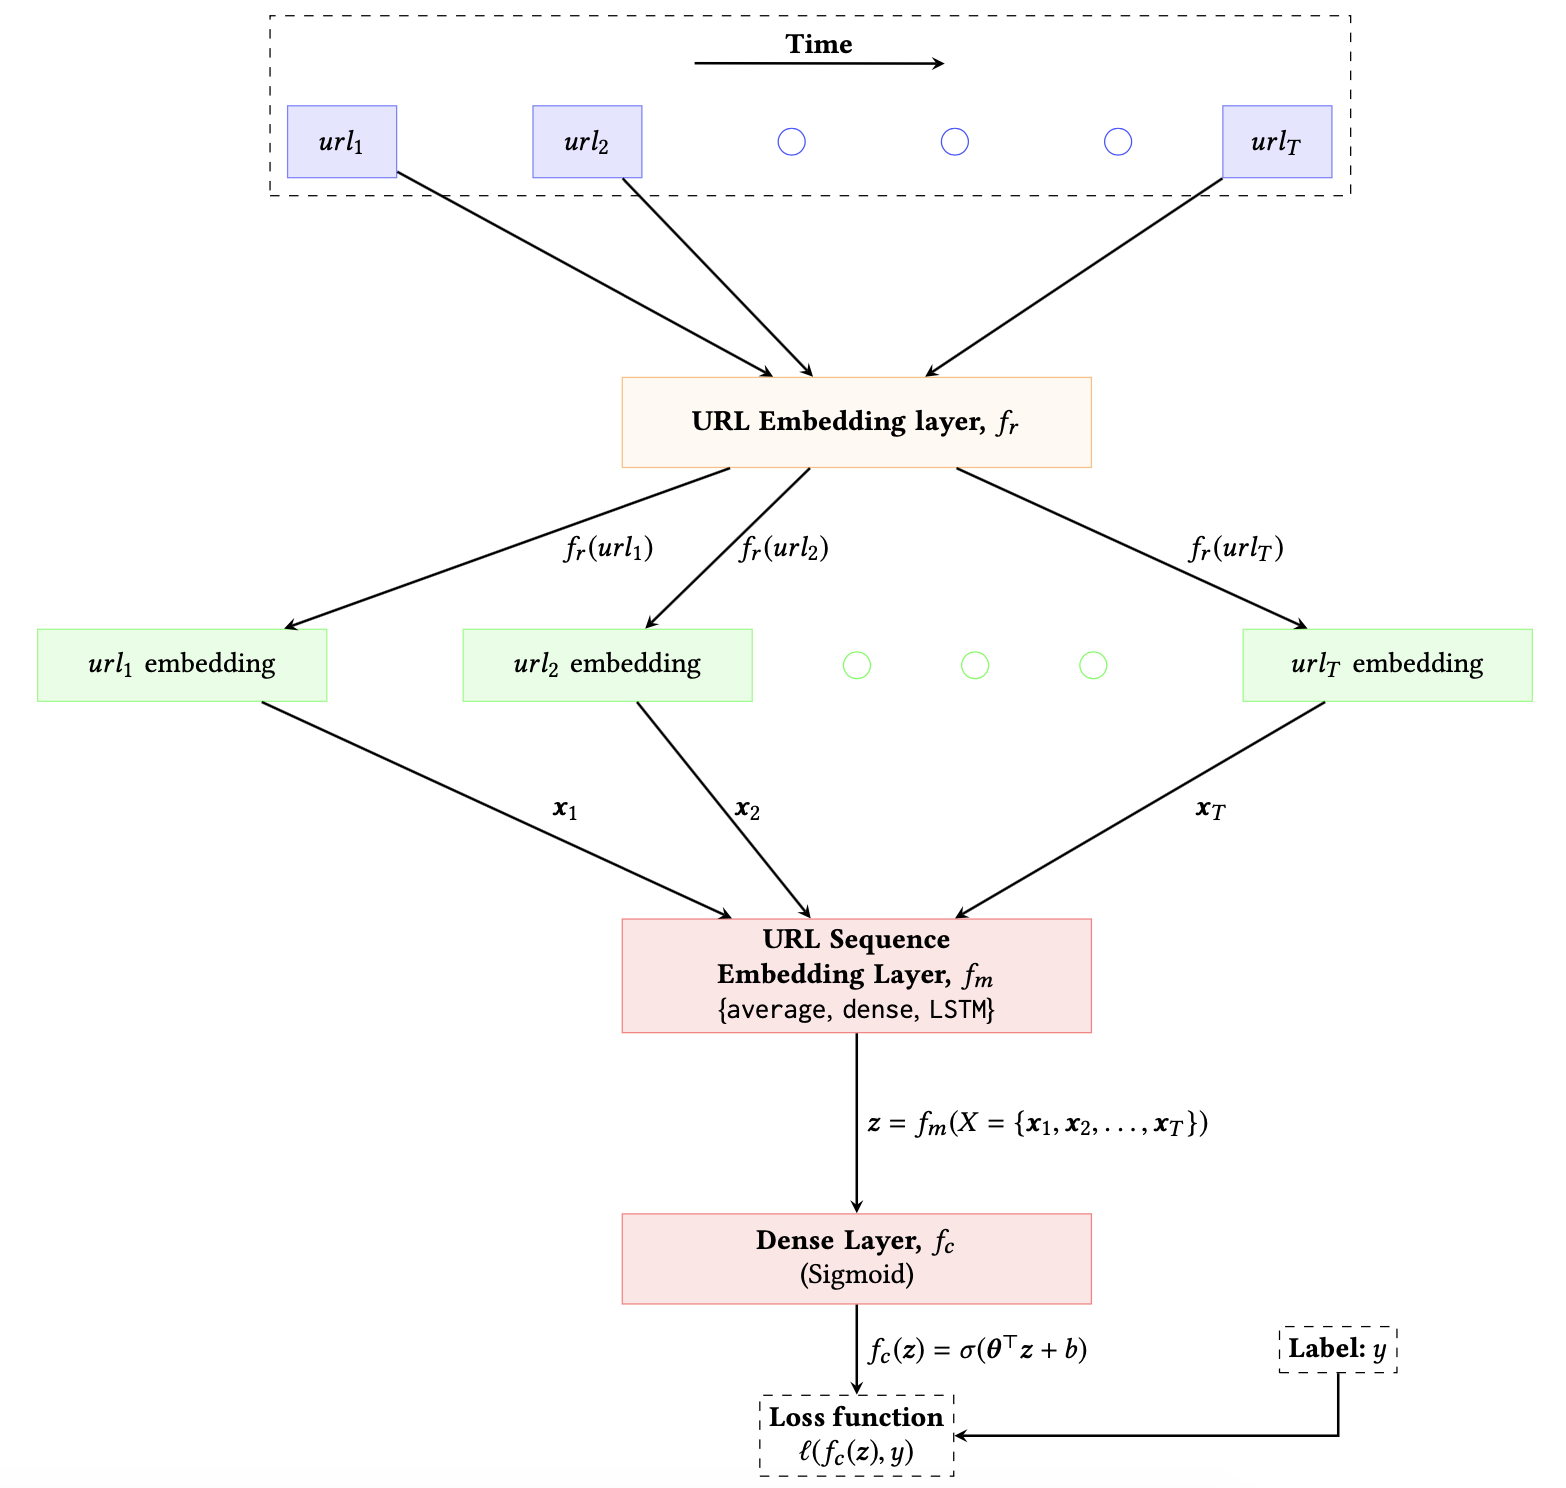
\includegraphics[width=0.8\linewidth]{images/predicting_conversions.png}
    \caption{Общая архитектура}
    \label{fig:predicting_conversion}
\end{figure}

\subsection{Experiments}

В рамках экспериментов, авторы оценивают качество разных комбинаций получения векторов URL'ов и получения фичей из истории пользователя.

Качество оценивают на задаче предсказания вероятности конверсии для пяти рекламодателей. В качестве метрики для оценки качества используют \texttt{ROC AUC}. \\

По результатм экспериментов лучше всего себя показала модель \texttt{Token\_avg/RNN}.

\section{Преимущества подхода}

\begin{itemize}
    \item Довольно прост в реализации
\end{itemize}

\section{Мое мнение}

\begin{itemize}
    \item Хотелось бы увидеть оценку качества на большем числе датасетов. Кажется, что сравнение на пяти рекламодателях это довольно мало для надежной оценки.
    \item Не смотря на то, что \texttt{Token\_avg/RNN} оказался лучшим по результатам оффлайн экспериментов, по метрикам видно, что baseline \texttt{One\_hot/LR} не так уж и сильно отстает по метрикам. Интересно было бы увидеть результаты сравнения данных моделей в онлайне
    \item Интересно почему авторы не используют дополнительную информацию о пользователях, а ограничились историей серфинга в интернете
    \item То что предлагают в статье очень похоже на то как я сейчас пробую сделать Lookalike
\end{itemize}